\begin{center} {\huge Supplementary material} \end{center}


\section{Data sources, patient selection, and study populations}

All analysis were performed in the NHS England (NHSE) Secure Data Environment (SDE) using patient level data from seven internally hosted datasets:

\begin{enumerate}
    \item \textit{Sentinel Stroke National Audit Programme (SSNAP)}: Acute stroke pathway data for first 72 hours of acute stroke care
    \item \textit{Demographics}: Date of death, sex, age group (5 years), ethnicity (5 categories)
    \item \textit{Office for National Statistics (ONS)}: Index of multiple deprivation (IMD) quintiles, Lower Super Output Area (LSOA), Rural and urban code 2011 (RUC11).
    \item \textit{Hospital Episode Statistics (HES)}: Days spent in care NHS inpatient care in the year after stroke, history of inpatient stroke admissions for the control patients
    \item \textit{Hometime}: Time spent alive, but outside of NHS inpatient care
    \item \textit{Covid infection \& vaccination}: Infection within 30 days and/or vaccination within 1 year of date of event
    \item \textit{Primary healthcare} (control patients only): history of stroke in primary care for the control patients
\end{enumerate} 

Data were retrieved for 388,506 emergency stroke admissions from an English LSOA, arriving at an acute stroke team in England between 01/01/2018 and 31/03/2023, obtained from SSNAP. SSNAP prospectively collects clinical data from 100\% of acute hospitals in England and Wales, with case ascertainment estimated at $>$90\% when compared with administrative coding data. Taking into account the framework used to transfer the SSNAP data to the NHSE SDE, features for the first 72 hours of the acute phase of the stroke pathway are included, up to and including any acute treatment (with thrombolysis and/or thrombectomy), excluding data about hospital transfer and hospital attended.

The analysis in this paper used four different study populations:

\begin{enumerate}
    \item The \emph{full exploratory population} of stroke patients (n = 388,345) contained patients who had a stroke and attended an acute stroke team. They had i) their stroke onset within 7 days of the arrival date range (133 patients were excluded), ii) their recorded procedures in the expected order of scan, then IVT, then MT (1 patient was excluded for scan after IVT, and 25 patients were excluded for MT after IVT).
    
    \item The \emph{eligible reperfusion treatment population} of stroke patients (n = 136,395) contained those who could be considered for emergency reperfusion stroke treatment. In addition to the full exploratory population filters above, these patients also i) arrived at an acute stroke team in England within 6 hours of stroke onset (208,381 patients were excluded), ii) had their stroke onset out of hospital (19,682 patients were excluded), iii) had an infarction (48,058 patients were excluded), iv) had a known stroke onset time (120,434 patients were excluded).
    
    \item The \emph{matched population - stroke patients} of stroke patients (n = 236,630) consisted of the set of stroke patients used to create a population of matched control patients. In addition to the full exploratory population filters above, these patients also i) had a matched control patient from primary records (14 patients were excluded; see following paragraph for matching protocol), ii) arrived at an acute stroke team in England from 01/11/2019 to remove survival bias for controls (144,551 patients were excluded), iii) had age recorded in SSNAP within 4 years of the age group recorded in the demographic dataset (3,731 patients were excluded), iv) had the same sex recorded in SSNAP and demographics (3,419 patients were excluded).

    \item The \emph{matched population - non-stroke patients} consisted of a population identified as not having had history of stroke in SSNAP, HES, or primary care records. A matched non-stroke patient was identified for each of the 236,630 stroke patients in the \textit{matched population - stroke patients}, matching on: i. age (5 year age band), ii. sex (male or female) and iii. ethnicity (categorized using 5 categories: 1) White; 2) Black, black British, African or Caribbean; 3) Mixed or multiple ethnic groups; 4) Asian or British Asian; 5) Other ethnic group) as recorded in the demographic dataset. The control patients lived in an English LSOA, were alive on the date their matched stroke patient had their stroke event (referred to onwards as the "date of event"), and did not have any history of stroke (recorded in the primary healthcare and HES dataset) prior to the date of event.
    
\end{enumerate}

For each patient (stroke and matched control), information was joined from the other four data sources (demographics, LSOA, hometime, and covid status). Stroke patients had 52 features describing their characteristics and the acute phase of the stroke pathway. The control patients had the features to describe their characteristics from all but the SSNAP dataset. Categorical features (such as ethnicity, covid status, treatment use/time, onset in hospital or arrival within 6 hours, stroke type, onset time type) were represented as one hot encoded features.

\subsection{Machine Learning methods}

\subsubsection{Model Choice}

We chose XGBoost (eXtreme Gradient Boosting) \cite{chen_xgboost_2016} as our primary model type. This is because XGBoost is  a fast, efficient, and performs excellently across different types of tabular data, with minimal tuning required \cite{shwartz-ziv_tabular_2022}. XGBoost allows for complex non-linear relations and feature-interactions in the data. XGBoost uses an ensemble of trees to make predictions. As such, XGBoost has poor explainability for any individual prediction. We added explainability by applying SHapley Additive exPlanations (SHAP) \cite{lundberg_consistent_2019} to the XGBoost output, to quantify the relative importance and directional effect of each clinical variable.

\subsubsection{Feature selection}

Features to included in the prediction XGBoost models were chosen based on four criteria: 1) identified as important to predict the outcome based on thrombolysis use \ref{pearn_thrombolysis_2026}, 2) used to filter patients in the causal model, 3) features identified by stakeholders, and 4) results of the sequential forward feature selection.

We used sequential forward feature selection to identify the features (from the 52 available features) to include in the model, with the motivation to create an explainable model with fewer features that still captured the majority of the accuracy. For each of the three location target features (in care, at home, dead) we trained XGBoost models on stratified 5-fold cross-validation data, sequentially selecting features to be included in the model as the single best feature to improve performance in terms of the R-squared. We repeated this process until model accuracy was equivalent (3 dp) to the model with all 52 features, or up to 25 features (whichever is greater).

For the \emph{reperfusion analysis cohort} of patients, we included treatment (use of thrombolysis or thrombectomy) and identified confounding factors (factors identified as being associated with both outcome directly, and with use of thrombolysis or thrombectomy) - these were 1. prior disability; 2. stroke severity on arrival; 3. age; 4. any atrial fibrilation diagnosis, 5. precise onset known (the directed acyclic graph , DAG, is shown in figure \ref{fig_dag}).

\begin{figure}
    \centering
    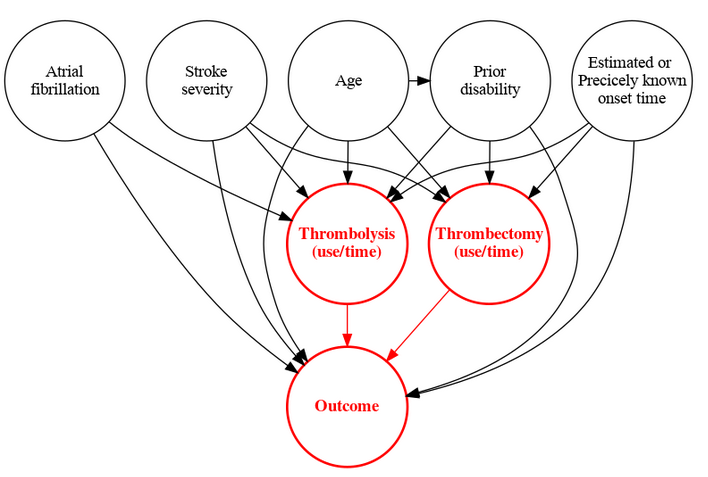
\includegraphics[width=0.7\linewidth]{images/output_results_from_SDE/dag_treatment_effect_on_first_year_location.png}
    \caption{DAG to isolate the effect of acute stroke treatment use/time on the first year following stroke.}
    \label{fig_dag}
\end{figure}


%%%%%%%%%%%%%%%%%%%%%%%%%%%%%%%%%%%%%%%%%%%%%%%%%%%%%%%%%%%%%%%%%%%%%%%%%%%%%

\section{Description of the stroke and matched control populations}

There are 236,630 instances in each of the matched populations (stroke and control populations). Table \ref{tab:stroke_control_011} shows the descriptive statistics of the main features.

\begin{table}[!ht]
    \centering
    \begin{tabular}{|l|l|l|l|}
    \hline
        \multicolumn{2}{|c|}{\bf Population cohort} & \bf Stroke & \bf Control \\ \hline
        \multicolumn{2}{|l|}{\bf Matched populations} & 236,630 & 236,630 \\ \hline
        \multirow{2}{*}{\bf Sex} & \bf Female & 110595 & 110595 \\
        & \bf Male & 126,035 & 126,035 \\ \hline
        \multirow{5}{*}{\bf Age, years} & \bf 0-20 & 130 & 240 \\
        & \bf 20-40 & 4460 & 5660 \\
        & \bf 40-60 & 36,915 & 42,565 \\
        & \bf 60-80 & 109,170 & 116,220 \\
        & \bf 80+ & 85,950 & 71,945 \\
        & \bf Mean [std] & 74 [13.7] & 71 [13.8] \\ \hline
        \multirow{5}{*}{\bf IMD quintiles (2019)} & \bf 1 & 48050 & 36155 \\
        & \bf 2 & 46,820 & 43,155 \\
        & \bf 3 & 48,305 & 49,680 \\
        & \bf 4 & 48,210 & 53,355 \\
        & \bf 5 & 45,250 & 54,285 \\ \hline
        \multirow{5}{*}{\bf Ethnicity} & \bf White & 213,240 & 213,240 \\
        & \bf Asian or Asian British & 12,160 & 12,160 \\
        & \bf Black, Black British, Caribbean or African & 6,545 & 6,545 \\
        & \bf Other ethnic group & 2,085 & 2,085 \\
        & \bf Mixed or multiple ethnic groups & 1,645 & 1,645 \\
        & \bf Unknown & 955 & 955 \\ \hline
        \multirow{4}{*}{\bf Covid} & \bf Infection only & 3,445 & 415 \\
        & \bf Vaccination only & 124,965 & 128,500 \\
        & \bf Vaccination and infection & 5,105 & 1,210 \\
        & \bf None & 103,115 & 106,510 \\ \hline
        \multirow{9}{*}{\bf Region} & \bf South East & 35,680 & 41,125 \\
        & \bf North West & 35,295 & 30,705 \\
        & \bf South West & 29,145 & 27,435 \\
        & \bf East of England & 26,160 & 27,965 \\
        & \bf Yorkshire and The Humber & 24,880 & 23,055 \\
        & \bf West Midlands & 24,275 & 25,085 \\
        & \bf London & 24,055 & 28,605 \\
        & \bf East Midlands & 22,390 & 21,120 \\
        & \bf North East & 14,750 & 11,535 \\ \hline
        \multirow{2}{*}{\bf Rural/urban (2011)} & \bf Urban & 188,895 & 185,025 \\
        & \bf Rural & 47,740 & 51,605 \\ \hline
    \end{tabular}
    \caption{Descriptive statistics of the main features for the 236,630 instances in the matched stroke and control populations. Counts to the nearest 5. Age of stroke patients was as recorded in SSNAP, while age of control patients was as recorded in demographic data (matching was performed using ages in demographic data)}.
    \label{tab:stroke_control_011}
\end{table}

%%%%%%%%%%%%%%%%%%%%%%%%%%%%%%%%%%%%%%%%%%%%%%%%%%%%%%%%%%%%%%%%%%%%%%%%%%

\section{Descriptive analysis (of impact of stroke on location)}

Figure \ref{fig:violin_location_365_days_post_stroke} shows that in the first year following a stroke, stroke patients spent, on average (mean), 266.4 days at home (138.6 standard deviation), 23.2 days in care (32.7 standard deviation) and 75.5 days dead (135.7 standard deviation). This was in comparison to the matched control population spending, on average (mean), 352.8 days at home (50.8 standard deviation), 2.4 days in care (10.2 standard deviation) and 9.8 days dead (48.0 standard deviation). When comparing individual matched patients, stroke patients spent, on average (mean), 86.4 days less at home (143.5 standard deviation), 20.8 more days in care (34.1 standard deviation), and died 65.7 days sooner (140.5 standard deviation). 
%ccu085_041_violinplot_365_days_post_stroke.png
\begin{figure}[ht]
\centering
 {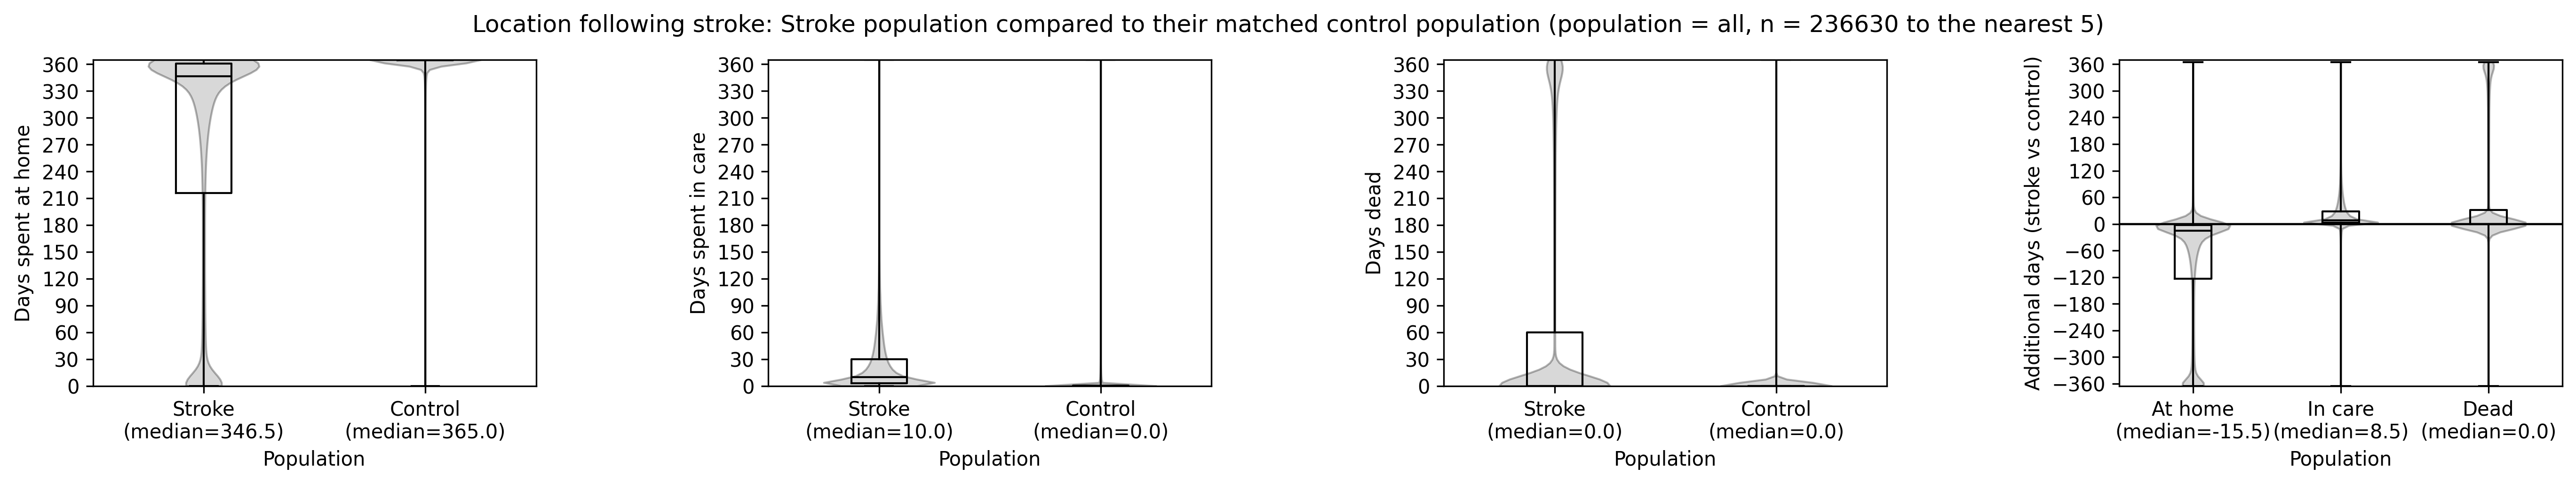
\includegraphics[width = 6.1in]{./images/output_results_from_SDE/ccu085_012_population_all_violinplot_365_days_post_stroke.png}}\\
 \caption{The distribution of the number of days the stroke patient population, and their matched control population, spent in each location in the year after stroke. LHS: Number of days spent at home. Left middle: Number of days spent in care. Right middle: Number of days dead. RHS: Additional days the stroke patient spent in comparison to their matched control.}
 \label{fig:violin_location_365_days_post_stroke}
\end{figure}

%%%%%%%%%%%%%%%%%%%%%

Table \ref{tab:stroke_location_post_stroke} shows that patients that have had a stroke use more healthcare resources in the year following their stroke if they are older, live in a more deprived area, have a more severe stroke, have a haemorrhage (rather than an ischaemic) stroke, or are Black, Black British, Caribbean or African. A stroke patient dies sooner if they are older, female, with unknown ethnicity, live in a less deprived area, or have a more severe stroke.

\newpage
\begin{landscape}
\begin{table}[!ht]
    \small
    \centering
    \begin{tabular}{|l|l|l|l|l|l|l|l|l|l|l|l|}
    \hline
        \multicolumn{2}{|c|}{\bf Population cohort} & \bf Count & \multicolumn{3}{|c|}{\bf At home} & \multicolumn{3}{|c|}{\bf In care} & \multicolumn{3}{|c|}{\bf Dead}\\ \hline
        \bf Feature name & \bf Feature value & \bf (nearest 5) & \bf mean & \bf std & \bf median & \bf mean & \bf std & \bf median & \bf mean & \bf std & \bf median \\ \hline
        \multicolumn{2}{|l|}{\bf Matched stroke population} & 236630 & 266.4 & 138.6 & 346.5 & 23.2 & 32.7 & 10.0 & 75.5 & 135.7 & 0.0 \\ \hline
        \multirow{3}{*}{\bf Age (years)} & \bf under 60 & 41510 & 325.1 & 86.5 & 359.0 & 19.5 & 37.0 & 5.5 & 20.4 & 78.4 & 0.0 \\ 
        & \bf 60-80 & 109170 & 286.7 & 124.9 & 352.0 & 22.6 & 33.4 & 8.5 & 55.6 & 121.1 & 0.0 \\
        & \bf over 80 & 85950 & 212.2 & 155.8 & 305.0 & 25.7 & 29.1 & 15.0 & 127.2 & 156.5 & 0.0 \\ \hline
        \multirow{2}{*}{\bf Sex} & \bf Female & 110595 & 253.4 & 144.7 & 339.5 & 23.7 & 31.3 & 11.0 & 87.9 & 143.3 & 0.0 \\ 
        & \bf Male & 126035 & 277.8 & 131.9 & 351.0 & 22.7 & 33.8 & 9.0 & 64.5 & 127.7 & 0.0 \\ \hline
        \multirow{6}{*}{\bf Ethnicity} & \bf Asian or Asian British & 12160 & 290.4 & 121.4 & 351.5 & 22.8 & 33.3 & 9.5 & 51.8 & 117.3 & 0.0 \\ 
        & \bf Black, Black British, Caribbean or African & 6545 & 287.0 & 118.7 & 346.0 & 30.5 & 43.4 & 13.5 & 47.5 & 112.1 & 0.0 \\
        & \bf Mixed or multiple ethnic groups & 1645 & 285.3 & 122.8 & 349.0 & 27.2 & 37.9 & 11.0 & 52.6 & 116.9 & 0.0 \\ 
        & \bf Other ethnic group & 2085 & 281.9 & 127.6 & 350.8 & 25.3 & 37.5 & 10.0 & 57.8 & 123.2 & 0.0 \\
        & \bf Unknown & 955 & 206.3 & 167.4 & 319.0 & 18.1 & 26.5 & 6.0 & 140.8 & 166.6 & 0.0 \\
        & \bf White & 213240 & 264.4 & 139.8 & 346.0 & 23.0 & 32.1 & 10.0 & 77.7 & 137.2 & 0.0 \\ \hline
        \multirow{5}{*}{\bf IMD} & \bf 1 & 48050 & 271.3 & 134.3 & 346.5 & 24.4 & 34.2 & 10.5 & 69.4 & 131.1 & 0.0 \\ 
        & \bf 2 & 46820 & 267.5 & 137.3 & 346.0 & 23.9 & 33.7 & 10.0 & 73.6 & 134.4 & 0.0 \\ 
        & \bf 3 & 48305 & 265.8 & 139.1 & 346.5 & 23.0 & 32.6 & 10.0 & 76.2 & 136.3 & 0.0 \\ 
        & \bf 4 & 48210 & 263.7 & 140.7 & 346.5 & 22.6 & 31.8 & 9.5 & 78.7 & 138.0 & 0.0 \\ 
        & \bf 5 & 45250 & 263.5 & 141.3 & 347.0 & 22.0 & 30.8 & 9.0 & 79.5 & 138.6 & 0.0 \\ \hline
        \multirow{4}{*}{\bf COVID} & \bf Infection only & 3445 & 221.6 & 153.6 & 312.0 & 32.0 & 39.3 & 18.0 & 111.4 & 155.2 & 0.0 \\
        & \bf None & 103115 & 268.7 & 137.7 & 347.5 & 22.1 & 31.2 & 9.5 & 74.2 & 135.0 & 0.0 \\
        & \bf Vaccination and infection & 5105 & 233.4 & 147.4 & 317.0 & 33.4 & 39.7 & 19.0 & 98.2 & 146.8 & 0.0 \\ 
        & \bf Vaccination only & 124965 & 267.0 & 138.1 & 347.0 & 23.4 & 33.2 & 10.0 & 74.6 & 135.1 & 0.0 \\ \hline
        \multirow{8}{*}{\bf Region} & \bf East Midlands & 22390 & 268.0 & 138.1 & 346.5 & 21.8 & 29.2 & 10.0 & 75.3 & 135.7 & 0.0 \\
        & \bf East of England & 26160 & 265.2 & 140.5 & 348.0 & 21.2 & 29.5 & 10.0 & 78.6 & 137.4 & 0.0 \\ 
        & \bf London & 24055 & 275.7 & 130.5 & 346.0 & 26.5 & 37.1 & 12.0 & 62.9 & 125.8 & 0.0 \\
        & \bf North East & 14750 & 268.6 & 138.4 & 348.0 & 21.8 & 32.2 & 8.5 & 74.7 & 135.4 & 0.0 \\
        & \bf North West & 35295 & 263.2 & 139.1 & 343.5 & 25.4 & 34.8 & 11.0 & 76.4 & 136.2 & 0.0 \\
        & \bf South East & 35680 & 266.4 & 138.6 & 347.5 & 22.9 & 32.7 & 9.5 & 75.7 & 136.1 & 0.0 \\
        & \bf South West & 29145 & 258.0 & 142.6 & 342.0 & 24.3 & 33.7 & 10.0 & 82.8 & 140.8 & 0.0 \\
        & \bf West Midlands & 24275 & 269.0 & 138.0 & 349.0 & 21.5 & 30.1 & 9.0 & 74.5 & 135.5 & 0.0 \\
        & \bf Yorkshire and The Humber & 24880 & 267.7 & 138.8 & 349.0 & 21.9 & 31.9 & 9.0 & 75.5 & 135.7 & 0.0 \\ \hline
        \multirow{2}{*}{\bf Rurality} & \bf Rural & 47740 & 264.1 & 140.8 & 347.0 & 22.0 & 31.4 & 9.0 & 78.9 & 138.4 & 0.0 \\ 
        & \bf Urban & 188895 & 267.0 & 138.0 & 346.0 & 23.5 & 33.0 & 10.0 & 74.6 & 135.0 & 0.0 \\ \hline
    \end{tabular}
    \caption{Number of days in the first year following the stroke event the matched stroke population spent in care, at home, or dead.}
    \label{tab:stroke_location_post_stroke}
\end{table}

\newpage
%\begin{landscape}
\begin{table}[!ht]
    \small
    \centering
    \begin{tabular}{|l|l|l|l|l|l|l|l|l|l|l|l|}
    \hline
        \multicolumn{2}{|c|}{\bf Population cohort} & \bf Count & \multicolumn{3}{|c|}{\bf At home} & \multicolumn{3}{|c|}{\bf In care} & \multicolumn{3}{|c|}{\bf Dead}\\ \hline
        \bf Feature name & \bf Feature value & \bf (nearest 5) & \bf mean & \bf std & \bf median & \bf mean & \bf std & \bf median & \bf mean & \bf std & \bf median \\ \hline
        \multicolumn{2}{|l|}{\bf Matched control population} & 236630 & 352.8 & 50.8 & 365.0 & 2.4 & 10.2 & 0.0 & 9.8 & 48.0 & 0.0 \\ \hline
        \multirow{3}{*}{\bf Age (years)} & \bf under 60 &  41510 & 363.8 & 14.5 & 365.0 & 0.5 & 5.3 & 0.0 & 0.7 & 12.9 & 0.0 \\
        & \bf 60-80 & 109170 & 359.3 & 33.8 & 365.0 & 1.6 & 8.6 & 0.0 & 4.1 & 31.3 & 0.0 \\
        & \bf over 80 & 85950 & 339.2 & 72.5 & 365.0 & 4.5 & 13.1 & 0.0 & 21.3 & 69.3 & 0.0 \\ \hline
        \multirow{2}{*}{\bf Sex} & \bf Female & 110595 & 351.3 & 53.6 & 365.0 & 2.7 & 10.4 & 0.0 & 11.0 & 51.0 & 0.0 \\
        & \bf Male & 126035 & 354.1 & 48.2 & 365.0 & 2.2 & 10.0 & 0.0 & 8.7 & 45.3 & 0.0 \\ \hline
        \multirow{6}{*}{\bf Ethnicity} & \bf Asian or Asian British & 12160 & 359.2 & 35.5 & 365.0 & 1.4 & 7.2 & 0.0 & 4.4 & 33.6 & 0.0 \\
        & \bf Black, Black British, Caribbean or African & 6545 & 359.4 & 34.6 & 365.0 & 1.4 & 8.3 & 0.0 & 4.2 & 32.2 & 0.0 \\
        & \bf Mixed or multiple ethnic groups & 1645 & 357.5 & 39.7 & 365.0 & 1.7 & 7.8 & 0.0 & 5.9 & 37.3 & 0.0 \\
        & \bf Other ethnic group & 2085 & 357.5 & 41.8 & 365.0 & 1.5 & 8.3 & 0.0 & 6.0 & 39.5 & 0.0 \\
        & \bf Unknown & 955 & 358.4 & 41.7 & 365.0 & 0.3 & 3.0 & 0.0 & 6.3 & 40.8 & 0.0 \\
        & \bf White & 213240 & 352.1 & 52.1 & 365.0 & 2.6 & 10.4 & 0.0 & 10.3 & 49.3 & 0.0 \\ \hline
        \multirow{5}{*}{\bf IMD} & \bf 1 & 36155 & 350.6 & 55.6 & 365.0 & 2.7 & 10.6 & 0.0 & 11.7 & 52.6 & 0.0 \\
        & \bf 2 & 43155 & 352.2 & 52.3 & 365.0 & 2.6 & 10.7 & 0.0 & 10.3 & 49.4 & 0.0 \\
        & \bf 3 & 49680 & 353.0 & 50.3 & 365.0 & 2.4 & 10.1 & 0.0 & 9.6 & 47.6 & 0.0 \\
        & \bf 4 & 53355 & 353.3 & 49.4 & 365.0 & 2.4 & 10.3 & 0.0 & 9.3 & 46.7 & 0.0 \\
        & \bf 5 & 54285 & 354.1 & 47.9 & 365.0 & 2.2 & 9.6 & 0.0 & 8.7 & 45.3 & 0.0 \\ \hline
        \multirow{4}{*}{\bf COVID} & \bf Infection only & 415 & 293.2 & 130.8 & 364.5 & 7.9 & 18.9 & 0.0 & 63.9 & 127.8 & 0.0 \\
        & \bf None & 106510 & 353.7 & 49.2 & 365.0 & 2.1 & 9.5 & 0.0 & 9.2 & 46.7 & 0.0 \\
        & \bf Vaccination and infection & 1210 & 328.1 & 91.7 & 365.0 & 6.6 & 20.5 & 0.0 & 30.3 & 86.4 & 0.0 \\
        & \bf Vaccination only & 128500 & 352.4 & 50.9 & 365.0 & 2.7 & 10.5 & 0.0 & 9.9 & 48.0 & 0.0 \\ \hline
        \multirow{9}{*}{\bf Region} & \bf East Midlands & 21120 & 352.8 & 50.4 & 365.0 & 2.4 & 9.2 & 0.0 & 9.9 & 47.9 & 0.0 \\
        & \bf East of England & 27965 & 353.2 & 49.6 & 365.0 & 2.4 & 9.9 & 0.0 & 9.4 & 46.9 & 0.0 \\
        & \bf London & 28605 & 354.9 & 46.6 & 365.0 & 2.2 & 9.5 & 0.0 & 8.0 & 43.7 & 0.0 \\
        & \bf North East & 11535 & 351.9 & 52.8 & 365.0 & 2.5 & 9.5 & 0.0 & 10.6 & 50.2 & 0.0 \\
        & \bf North West & 30705 & 352.2 & 51.9 & 365.0 & 2.8 & 11.8 & 0.0 & 10.0 & 48.6 & 0.0 \\
        & \bf South East & 41125 & 353.0 & 50.6 & 365.0 & 2.3 & 9.9 & 0.0 & 9.7 & 47.9 & 0.0 \\
        & \bf South West & 27435 & 352.1 & 52.3 & 365.0 & 2.6 & 11.3 & 0.0 & 10.3 & 49.5 & 0.0 \\
        & \bf West Midlands & 25085 & 352.4 & 51.5 & 365.0 & 2.5 & 9.9 & 0.0 & 10.1 & 48.7 & 0.0 \\
        & \bf Yorkshire and The Humber & 23055 & 352.0 & 52.9 & 365.0 & 2.3 & 9.6 & 0.0 & 10.7 & 50.3 & 0.0 \\ \hline
        \multirow{2}{*}{\bf Rurality} & \bf Rural & 51605 & 353.4 & 49.9 & 365.0 & 2.3 & 10.2 & 0.0 & 9.3 & 47.2 & 0.0 \\
        & \bf Urban & 185025 & 352.6 & 51.1 & 365.0 & 2.5 & 10.2 & 0.0 & 9.9 & 48.3 & 0.0 \\ \hline
    \end{tabular}
    \caption{Number of days in the first year following the stroke event the matched control population spent in care, at home, or dead.}
    \label{tab:control_location_post_stroke}
\end{table}


\begin{table}[!ht]
    \centering
    \begin{tabular}{|l|l|l|l|l|l|l|l|l|l|l|l|}
    \hline
        \multicolumn{2}{|c|}{\bf Population cohort} & \bf Count & \multicolumn{3}{|c|}{\bf At home} & \multicolumn{3}{|c|}{\bf In care} & \multicolumn{3}{|c|}{\bf Dead}\\ \hline
        \multicolumn{2}{|c|}{} & \bf Nearest 5 & \bf mean & \bf std & \bf median & \bf mean & \bf std & \bf median & \bf mean & \bf std & \bf median \\ \hline
        \multicolumn{2}{|l|}{\bf Whole population} & 236630 & -86.4 & 143.5 & -15.5 & 20.8 & 34.1 & 8.5 & 65.7 & 140.5 & 0 \\ \hline
        \bf Feature name & \bf Feature value & & & & & & & & & & \\ \hline
        \multirow{3}{*}{\bf Age (years)} & \bf under 60  &  41510 & -38.7 & 87.8 & -6.0 & 19.0 & 37.4 & 5.0 & 19.7 & 79.6 & 0\\
        ~ & \bf 60-80 & 109170 & -72.6 & 128.9 & -11.5 & 21.1 & 34.5 & 8.0 & 51.5 & 124.7 & 0 \\ 
        ~ & \bf over 80 & 85950 & -127.1 & 169.8 & -48.0 & 21.2 & 31.9 & 12.5 & 105.9 & 169.2 & 0 \\ \hline
        \multirow{2}{*}{\bf Sex} & \bf Female & 110595 & -97.9 & 150.1 & -21.5 & 21.1 & 32.8 & 10.0 & 76.9 & 148.5 & 0 \\ 
        ~ & \bf Male & 126035 & -76.3 & 136.6 & -12.0 & 20.5 & 35.1 & 7.5 & 55.8 & 132.3 & 0 \\ \hline
        \multirow{6}{*}{\bf Ethnicity} & \bf Asian or Asian British & 12160 & -68.8 & 124.8 & -12.5 & 21.5 & 34.0 & 9.0 & 47.3 & 120.5 & 0 \\ 
        ~ & \bf Black, Black British, Caribbean or African & 6545 & -72.4 & 121.3 & -17.5 & 29.1 & 44.2 & 13.0 & 43.4 & 114.6 & 0 \\
        ~ & \bf Mixed or multiple ethnic groups & 1645 & -72.2 & 122.6 & -14.5 & 25.5 & 38.5 & 10.0 & 46.7 & 116.8 & 0 \\ 
        ~ & \bf Other ethnic group & 2085 & -75.6 & 132.0 & -13.0 & 23.8 & 38.3 & 9.0 & 51.8 & 127.0 & 0 \\ 
        ~ & \bf Unknown & 955 & -152.1 & 169.6 & -43.0 & 17.7 & 26.7 & 6.0 & 134.5 & 168.7 & 0 \\
        ~ & \bf White & 213240 & -87.8 & 145.0 & -16.0 & 20.4 & 33.6 & 8.5 & 67.4 & 142.2 & 0 \\ \hline
    \end{tabular}
    \caption{Number of additional days in the first year following the stroke event the stroke patient spends in each location compared to their pairwise matched control patient (showing data for the matched features).}
    \label{tab:stroke_v_control_location_post_stroke}
\end{table}

\end{landscape}

\subsection{Survival analysis following stroke}

We defined the baseline characteristics of a patient to be: white; under 60 years old; living in the 20\% most deprived area; had no covid vaccination within 12 months of stroke event; had no covid infection within 30 days of stroke event; receive no acute treatment (thrombolysis or thrombectomy), no diabetes, no arterial fibrillation, precisely known onset time, infarction, onset out of hospital and arrive within 6 hours. The survival rate of the baseline stroke patient for the exploratory population and the causal population in the first year following a stroke event is shown in figure \ref{survival_baseline}. Within 50 days of their stroke 10.5\% of the full exploratory stroke population have died, and 22.0\% being dead by the end of the first year following their stroke. In comparison, 9.3\% of the causal stroke population have died within the first year of the stroke event, and 19.9\% being dead at the end of the first year following their stroke.

\begin{figure}[ht]
  \centering
  \subfloat[Full exploratory population.]{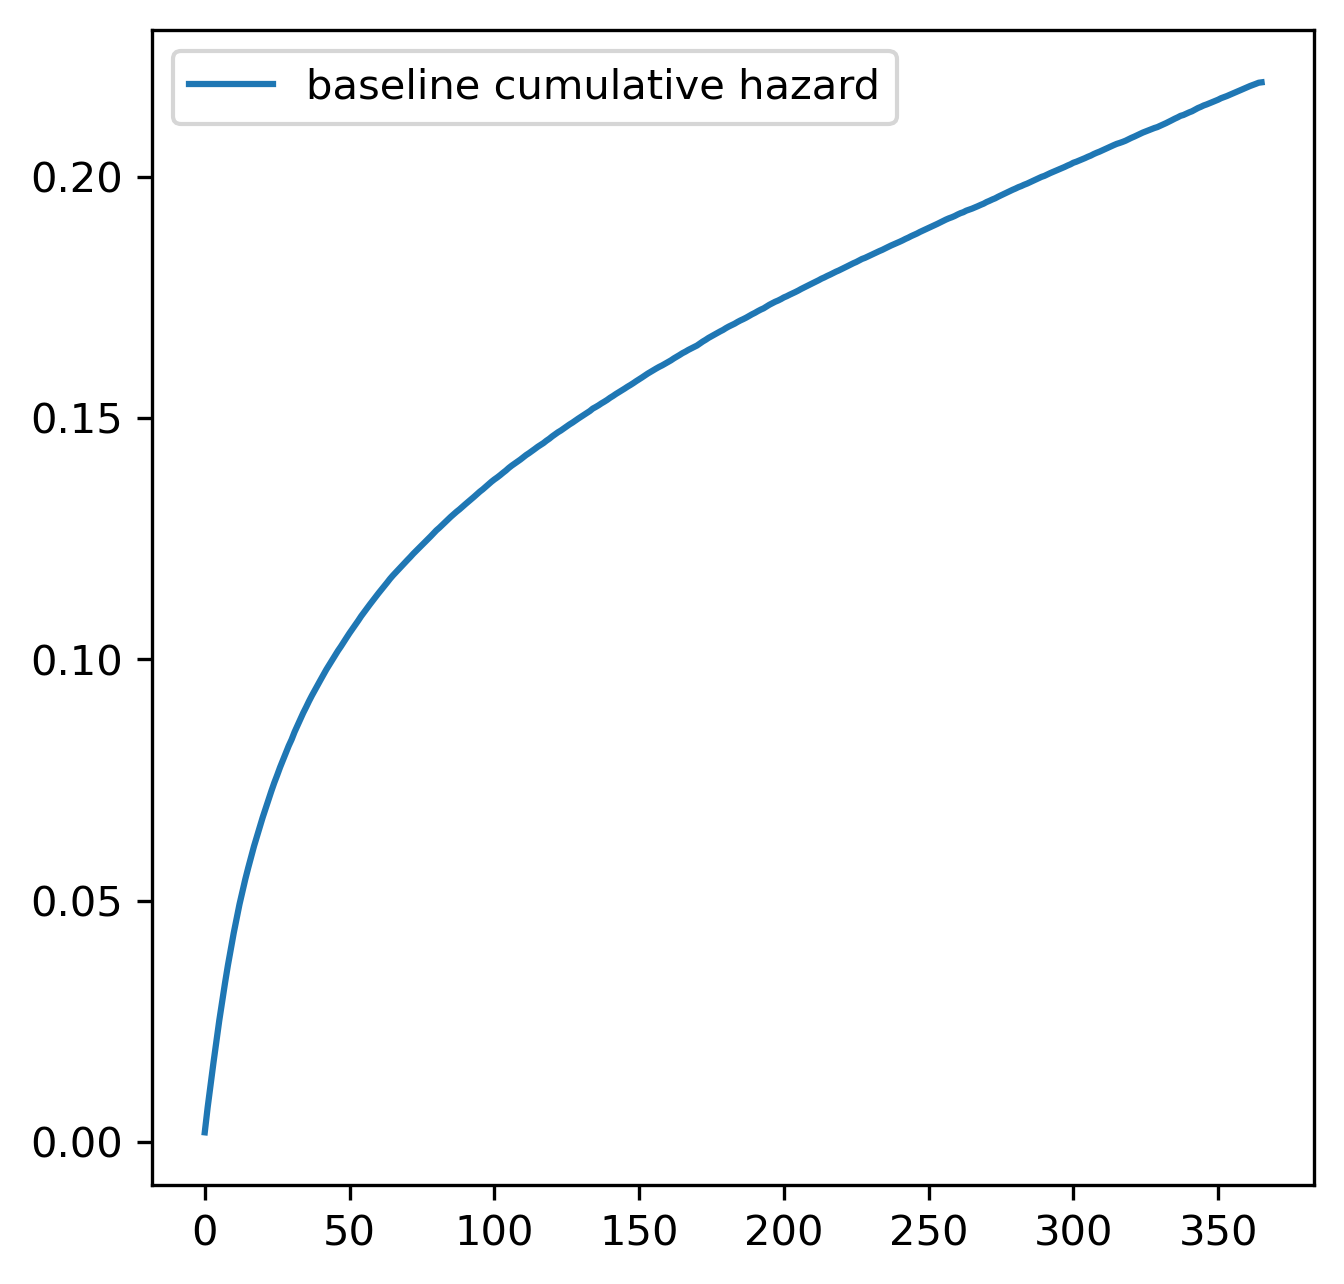
\includegraphics[width=0.4\textwidth]{./images/output_results_from_SDE/ccu085_040_baseline_hazard_from_cox_proportional_hazard_ratio_model_survival_in_year_following_stroke_exploratory_population.png}\label{stroke_survival_baseline}}
  \hfill
  \subfloat[Causal population.]{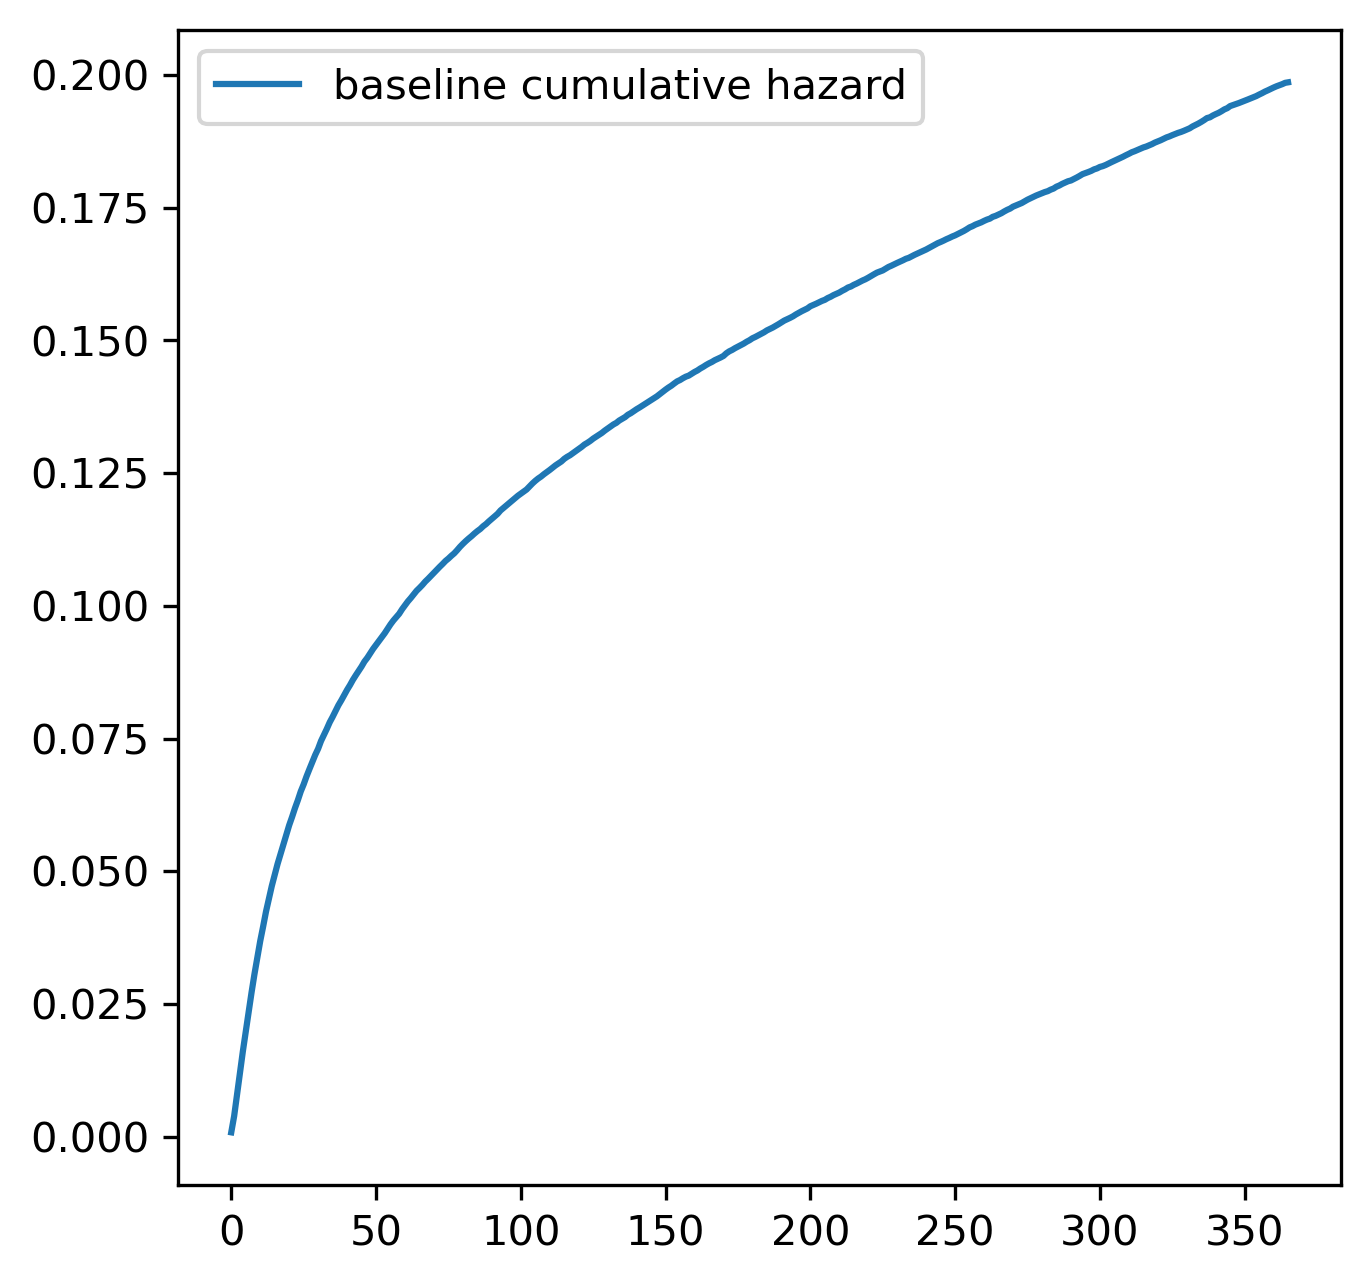
\includegraphics[width=0.4\textwidth]{./images/output_results_from_SDE/ccu085_050_baseline_hazard_from_cox_proportional_hazard_ratio_model_survival_in_year_following_stroke_causal_population.png}\label{control_survival_baseline}}
  \caption{Baseline survival rate in the first year following the stroke event for a baseline patient (white, under 60 years old, living in the most deprived 20\% area, had no covid vaccination within 12 months of stroke event, had no covid infection within 30 days of stroke event, receive no acute treatment (thrombolysis or thrombectomy), no diabetes, no atrial fibrilation, ischaemic stroke, onset outside of hospital and arrived within 6 hours. LHS shows the stroke exploratory population, RHS shows the stroke causal population (where all patients had an ischaemic stroke onset out of hospital and arrived within 6 hours of onset).\label{survival_baseline}}
\end{figure}

The effect of a patients characteristics deviating from this defined baseline stroke patient (for each population: exploratory and causal) are shown as hazard ratios for each feature as a forest plot (figure \ref{fig:forest_plot}) with the features ranked by impact on survival (see also table \ref{tab:hazard_ratios}).

%%%%%%%%%%%%%%%%%%%%%%%%%%%%%%%%%%%%%%%%%%%%%%%%%%%%%%%%%%%%%%%%%%%%%%%%%%%%

\subsubsection{Feature selection}

Table \ref{tab:feature-selection} shows sequential forward feature selection for each of the three models. Sequential forward feature selection is a greedy algorithm that starts with no features and iteratively adds the feature that most improves a model’s performance until a stopping criterion is met (in this case 25 features were selected, and performance then compared with using all available 52 features).

\begin{landscape}

\begin{table}[!ht]
    \small
    \centering
    \begin{tabular}{|l|l|l|l|l|l|l|}
    \hline
        ~ & \multicolumn{2}{|c|}{\bf In care} & \multicolumn{2}{|c|}{\bf At home} & \multicolumn{2}{|c|}{\bf Dead}\\ \hline
        \bf Number of features & \bf Feature & \bf r2 & \bf Feature & \bf r2 & \bf Feature & \bf r2  \\ \hline
        \bf 1 & stroke\_severity\_arrival & 0.066 & stroke\_severity\_arrival & 0.258 & stroke\_severity\_arrival & 0.226 \\ \hline
        \bf 2 & prior\_disability & 0.093 & age & 0.330 & age & 0.304 \\ \hline
        \bf 3 & arrival\_to\_scan\_time\_mins & 0.104 & prior\_disability & 0.354 & prior\_disability & 0.325 \\ \hline
        \bf 4 & age & 0.114 & thrombolysis\_no\_but\_haemorrhagic & 0.364 & thrombolysis\_no\_but\_haemorrhagic & 0.336 \\ \hline
        \bf 5 & onset\_to\_su\_arrival\_time\_mins & 0.124 & arrival\_to\_scan\_time\_mins & 0.373 & onset\_in\_hospital & 0.339 \\ \hline
        \bf 6 & thrombolysis\_no\_but\_haemorrhagic & 0.130 & arrival\_to\_thrombolysis\_time\_mins & 0.376 & eth5 & 0.342 \\ \hline
        \bf 7 & onset\_to\_scan\_time\_mins & 0.134 & eth5 & 0.378 & arrival\_to\_thrombolysis\_time\_mins & 0.345 \\ \hline
        \bf 8 & region & 0.136 & male & 0.380 & afib\_anticoagulant & 0.346 \\ \hline
        \bf 9 & arrive\_by\_ambulance & 0.138 & onset\_to\_su\_arrival\_time\_mins & 0.382 & onset\_to\_su\_arrival\_time\_mins & 0.348 \\ \hline
        \bf 10 & scan\_to\_thrombolysis\_time\_mins & 0.140 & onset\_to\_scan\_time\_mins & 0.384 & onset\_time\_type & 0.350 \\ \hline
        \bf 11 & arrival\_to\_thrombectomy\_time\_mins & 0.141 & arrive\_by\_ambulance & 0.386 & atrial\_fibrillation & 0.352 \\ \hline
        \bf 12 & tia\_last\_month & 0.141 & arrival\_to\_thrombectomy\_time\_mins & 0.387 & male & 0.353 \\ \hline
        \bf 13 & thrombolysis\_to\_thrombectomy\_time\_mins & 0.141 & afib\_doac\_anticoagulant & 0.389 & thrombolysis\_no\_but\_comorbidity & 0.354 \\ \hline
        \bf 14 & arrival\_to\_thrombolysis\_time\_mins & 0.141 & atrial\_fibrillation & 0.390 & diabetes & 0.355 \\ \hline
        \bf 15 & thrombolysis\_no\_but\_age & 0.142 & diabetes & 0.391 & arrival\_to\_thrombectomy\_time\_mins & 0.356 \\ \hline
        \bf 16 & diabetes & 0.142 & thrombolysis\_no\_but\_improving & 0.392 & arrive\_by\_ambulance & 0.357 \\ \hline
        \bf 17 & thrombolysis\_no\_but\_toomildsevere & 0.143 & congestive\_heart\_failure & 0.393 & stroke\_type & 0.358 \\ \hline
        \bf 18 & afib\_heparin\_anticoagulant & 0.143 & inr\_arrival & 0.393 & prior\_stroke\_tia & 0.358 \\ \hline
        \bf 19 & male & 0.143 & thrombolysis\_no\_but\_othermedical & 0.393 & thrombolysis\_no\_but\_toomildsevere & 0.359 \\ \hline
        \bf 20 & eth5 & 0.143 & new\_afib\_diagnosis & 0.393 & thrombolysis\_to\_thrombectomy\_time\_mins & 0.359 \\ \hline
        \bf 21 & prior\_stroke\_tia & 0.145 & thrombolysis\_no\_but\_age & 0.393 & new\_afib\_diagnosis & 0.359 \\ \hline
        \bf 22 & thrombolysis\_no\_but\_improving & 0.144 & afib\_vit\_k\_anticoagulant & 0.394 & afib\_antiplatelet & 0.359 \\ \hline
        \bf 23 & thrombolysis\_no\_but\_medication & 0.145 & region & 0.393 & inr\_arrival & 0.359 \\ \hline
        \bf 24 & recent\_covid & 0.145 & afib\_heparin\_anticoagulant & 0.394 & afib\_doac\_anticoagulant & 0.359 \\ \hline
        \bf 25 & inr\_arrival & 0.145 & thrombolysis\_no\_but\_refusal & 0.394 & hypertension & 0.360 \\ \hline
        \multicolumn{7}{|l|}{\bf Additional results} \\ \hline
        \bf 52 & All 52 features & 0.143 & ~ & 0.394 & ~ & 0.359 \\ \hline
        \bf 12 & 12 chosen features & 0.120 & ~ & 0.380 & ~ & 0.347 \\ \hline
    \end{tabular}
    \caption{Results of the sequential feature selection for the XGBoost models, a separate one predicting the duration spent i. in care ii. at home iii. dead in the first year following a stroke. The feature giving the best mean R-squared across the 5 k-folds are sequentially selected. Also reported are the results for a model with all 52 features, and the 12 features chosen for the prediction XGBoost models.}
    \label{tab:feature-selection}
\end{table}

\end{landscape}

We selected 12 features to be included in each of the prediction XGBoost models based on four criteria:

\textbf{Criteria A. Predictive of thrombolysis use (\cite{pearn_thrombolysis_2026}}

\begin{enumerate}
  \setcounter{enumi}{0}
    \item Acute treatment use/time: Represented as a categorical feature with 8 levels, using 4.5 hours from onset of stroke to treatment as the early/late cutoff (no treatment, only early IVT, only late IVT, early IVT and MT, early IVT and late MT, late IVT and late MT, only early MT, only late MT).
    \item Prior disability level: Disability level (mRS) before stroke
    \item Stroke severity: Stroke severity (NIHSS) on arrival
    \item Age: Middle of 5 year age bands
    \item Any atrial fibrillation diagnosis: Patient has a diagnosis of atrial fibrillation (either previously diagnosed or new)
    \item Onset time type: Onset time recorded is precise time, a best estimate or not known   
\end{enumerate}

\textbf{Criteria B. Used to filter patients in the causal model}

\begin{enumerate}
  \setcounter{enumi}{6}
    \item Onset in hospital or arrival within 6 hours: Combines onset in hospital and onset to arrival features into a single categorcial feature with 3 levels (onset in hospital, arrival within 6 hours, arrival beyond 6 hours)
    \item Stroke type: Ischaemic, haemorragic, not known.
\end{enumerate}

\textbf{Criteria C. Feature selection results}
\begin{enumerate}
  \setcounter{enumi}{8}
    \item Diabetes (binary)
    \item Ethnicity: 5 categorical level
\end{enumerate}

\textbf{Criteria D: Features we are interested in}
\begin{enumerate}
  \setcounter{enumi}{10}
    \item IMD quintiles (2019): Where 1 is most deprived, and 5 is least deprived
    \item Covid status: Categorical feature with 4 levels, using 30 days to define whether a patient had a covid infection, and 12 months to define whether a patient is in the covid vaccinated cohort  at the time of the date of event (vaccinated and infected, just vaccinated, just infected, neither).    
\end{enumerate}

A model using these 12 features was able to provide 84.4\%, 96.5\% and 96.8\% of the accuracy obtained when all 52 features were used (mean R-squared across the 5 k-folds for 12 vs 52 features (for in care, at home and dead respectively): 12.0 vs 14.3, 38.0 vs 39.4, 34.7 vs 35.9). Correlations between the 12 features were measured - they were largely independent of each other \ref{Fig:correlation_matrix}. Ignoring comparisons between levels from the same one hot encoded feature, all R-squared were less than 0.05 except (a) arrive within 6 hours and acute treatment (R-squared 0.14 with no treatment, 0.12 with only early IVT), (b) prior disability level and age (0.13), (c) onset time type and acute treatment (precisely known onset time and no treatment 0.11, precisely known onset time and only early IVT 0.10, onset unknown and no treatment 0.05), (d) age and any atrial fibrillation diagnosis (0.08), (e) prior disability level and stroke severity (R-squared 0.06).

\begin{figure}[!htb]
\hspace*{0cm}
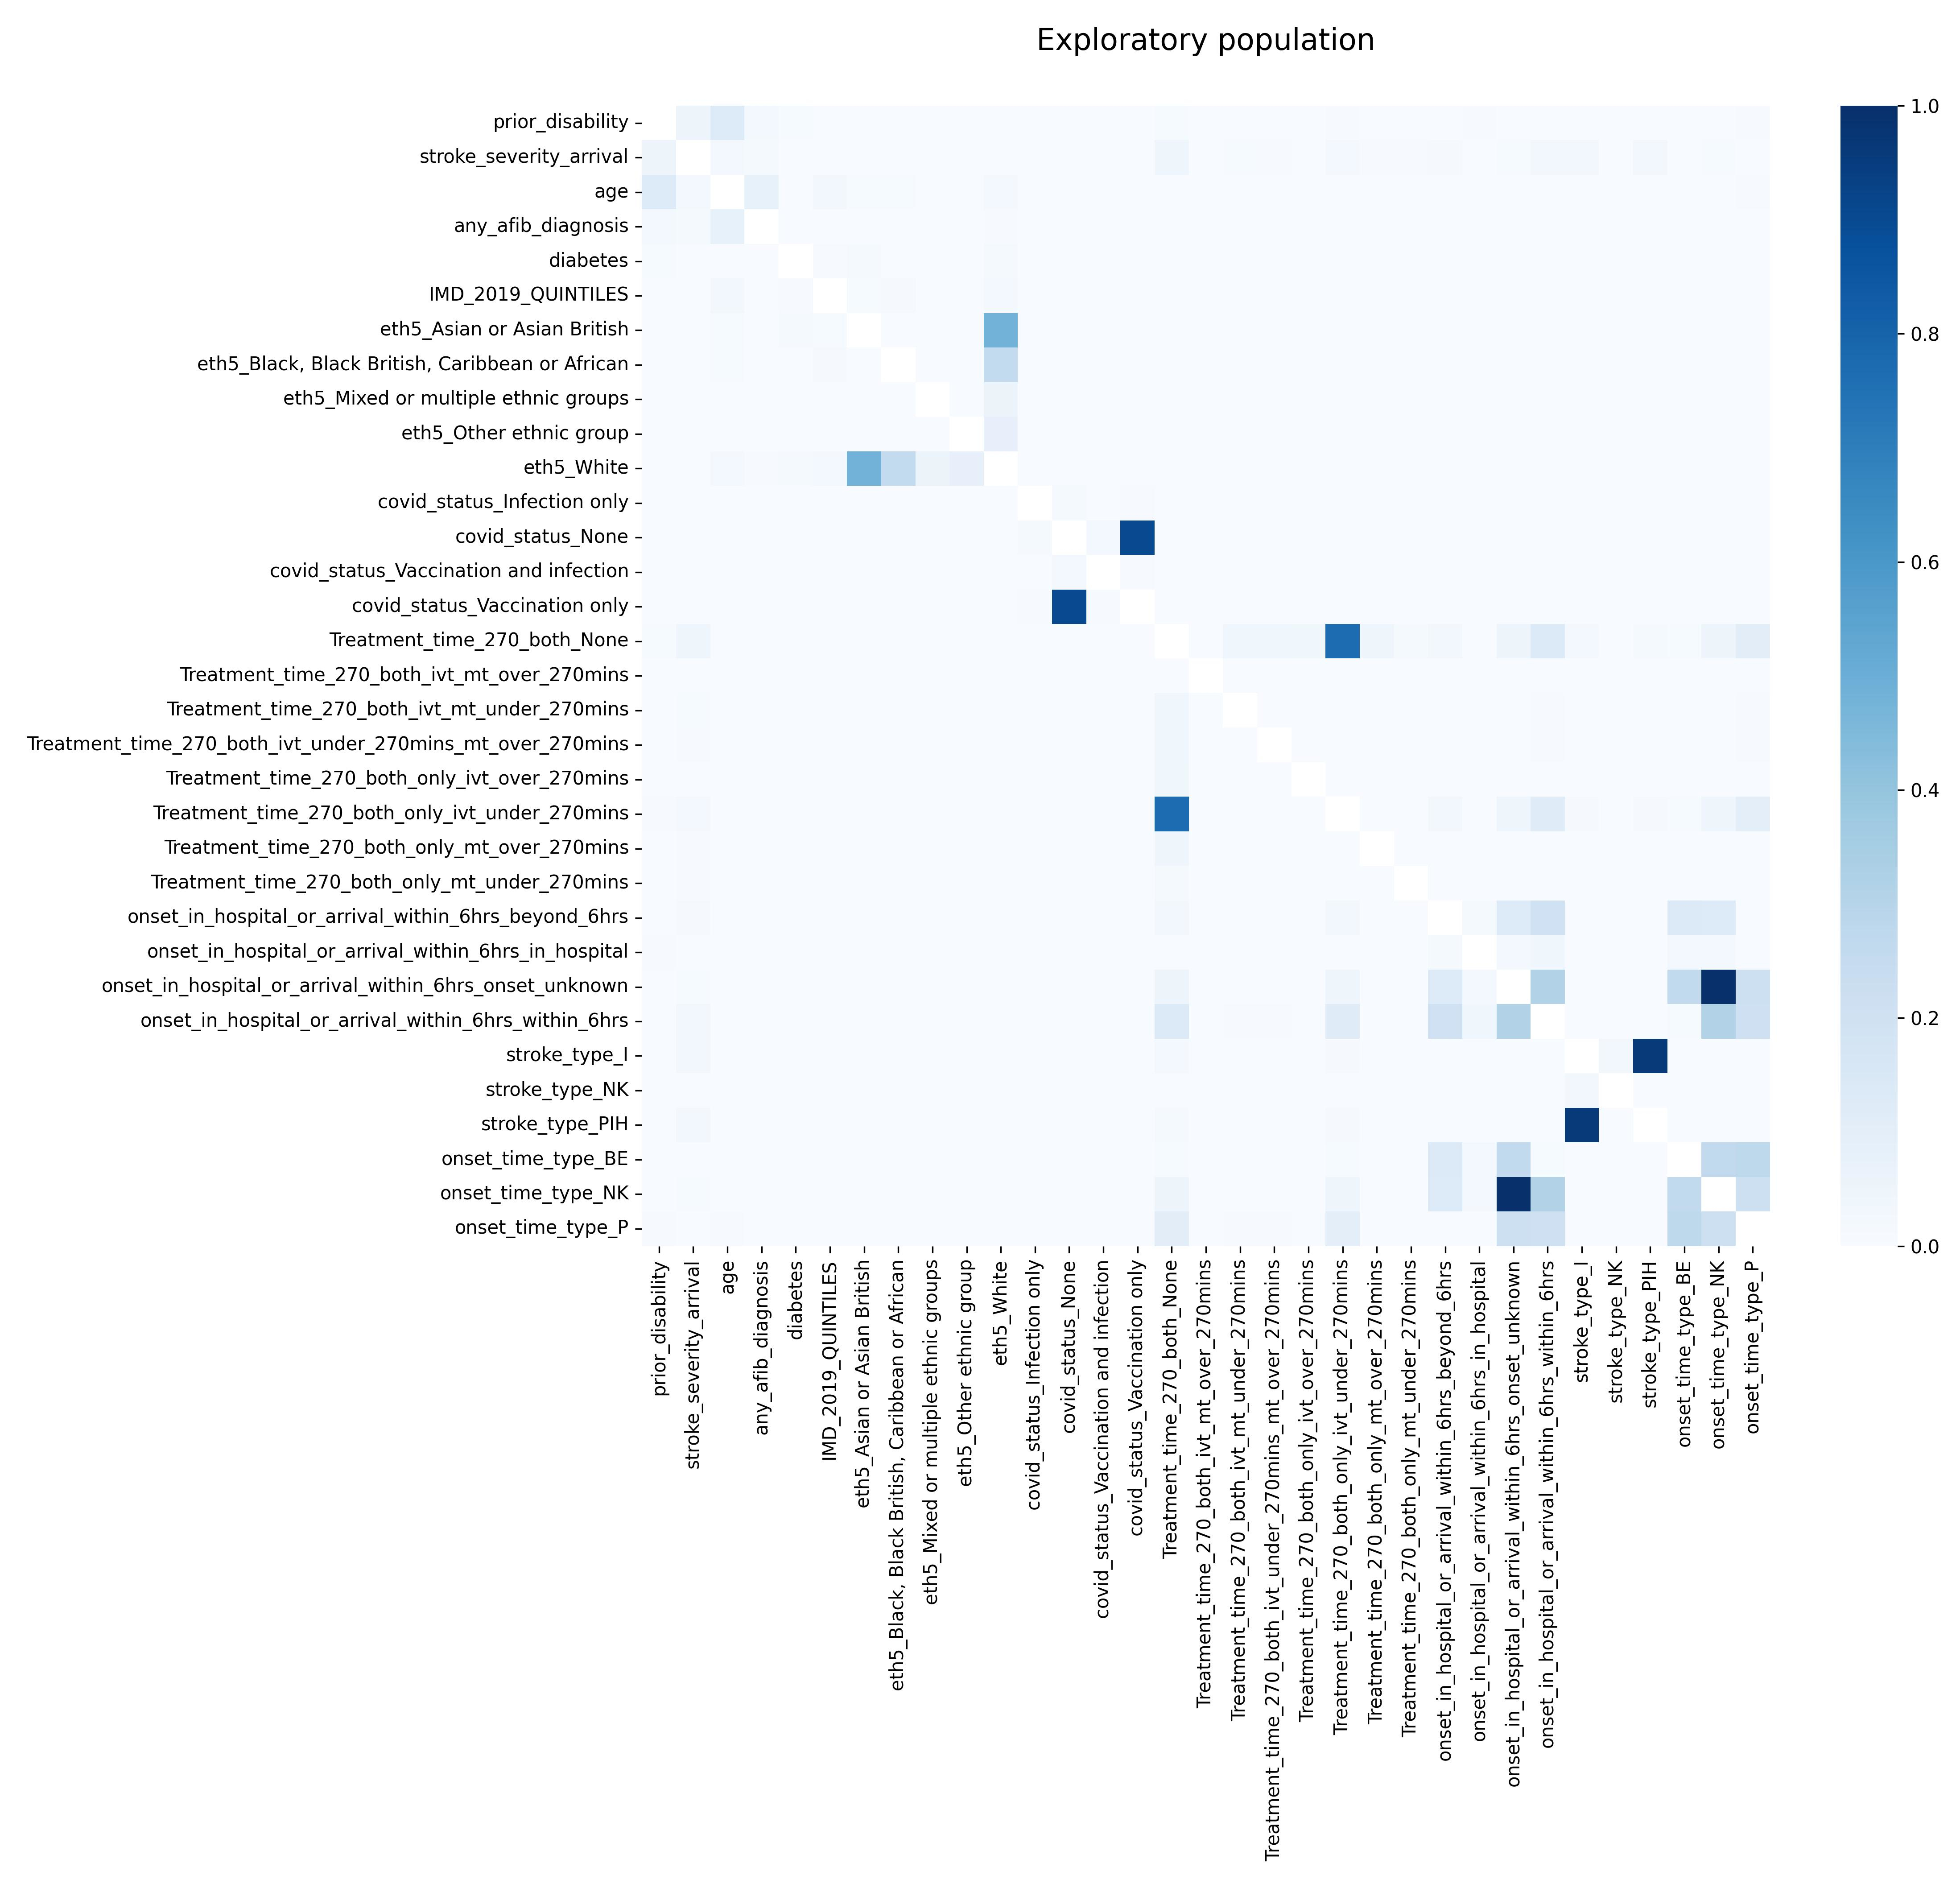
\includegraphics[trim=0 0 0 30,clip,width=\textwidth]{images/output_results_from_SDE/178_correlation_heatmap_exploration.jpg}%
\hspace*{0.05cm}
\caption{Correlation matrix between the 12 features for the full exploratory population (with categorical features represented as OHE features).}
\label{Fig:correlation_matrix}
\end{figure}

